\newpage
\section{Картотека пациентов}

В \tmis ~для каждого пациента заводится регистрационная карточка, которая содержит всю персональную информацию о пациенте. Она регистрируется в системе при первичном обращении пациента в ЛПУ (одновременно с заведением амбулаторной карты или истории болезни). При всех последующих обращениях осуществляется поиск ранее зарегистрированной карточки пациента и привязка к ней очередного случая обращения. В случае изменения каких-либо персональных данных пациента, регистрационную карточку можно отредактировать. 

Таким образом, регистрация пациента в системе аналогично заведению медицинской карты амбулаторного больного в поликлинике, когда паспортная часть карты оформляется один раз, а медицинские записи добавляются в нее при каждом обращении. \tmis~ позволяет использовать единую регистрационную карточку не только для поликлиники, но и для стационара, что значительно упрощает процедуру оформления истории болезни при направлении пациента из поликлиники или при повторной госпитализации. Благодаря данному механизму так же значительно упрощается получение врачом медицинской информации о предыдущих случаях обращения пациента.

Совокупность регистрационных карточек пациентов, случаев их обращений в ЛПУ и результатов обращений называется картотекой пациентов. Для доступа к картотеке пациентов необходимо в главном меню выбрать пункт \mm{Работа~\str Обслуживание пациентов}. На вкладке \dm{Пациенты} открывшегося окна можно найти нужного пациента или зарегистрировать нового. На вкладке \dm{Обращение} можно получить подробную информацию обо всех обращениях пациента или зарегистрировать новое обращение. На вкладке \dm{Обслуживание} содержится информация обо всех медицинских записях, сделанных в составе различных обращений.

\subsection{Поиск регистрационной карточки пациента} \label{cl_find}

Поиск, регистрация, редактирование регистрационных карточек пациентов осуществляется на вкладке \dm{Пациенты} окна обслуживания пациентов (Рисунок \ref{img_cl_find}). Если часть полей не умещается на экране, можно воспользоваться полосой прокрутки для перемещения в нужную часть окна.

\begin{figure}[ht]\centering
 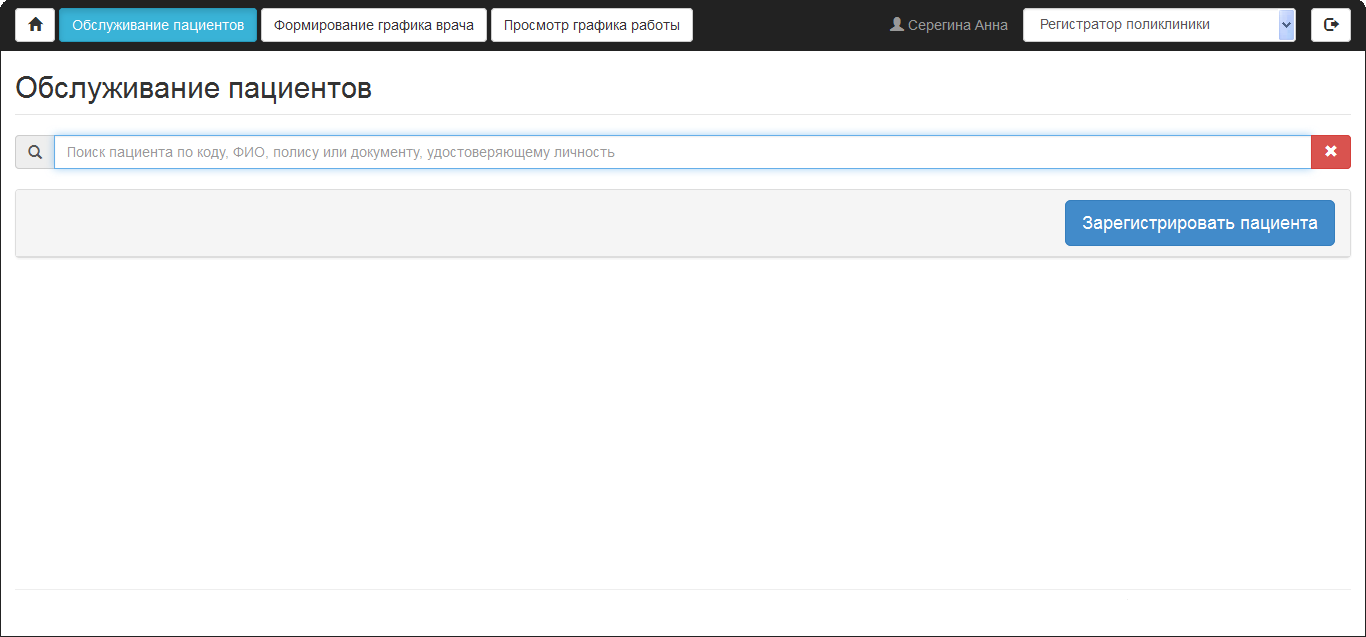
\includegraphics[width = 1\textwidth ,keepaspectratio]{cl_find}
 \caption{Окно работы с регистрационными карточками пациентов}
 \label{img_cl_find}
\end{figure} 

Вкладку \dm{Пациенты} условно можно разделить на 6 секций (Рисунок \ref{img_cl_find}):
\begin{itemize}
 \item В секции 1 представлены основные данные пациента, на регистрационной карточке которого в текущий момент установлен курсор в секции 2. Поле носит информационный характер, редактирование данных в нем невозможно.
 \item В секции 2 отображается список пациентов. Он может быть полным или ограниченным условиями фильтра (секция 3). Если список слишком большой, то отображаются первые 10 000 записей. Для поиска пациента в списке рекомендуется использовать фильтрацию.
 \item В секции 3 расположены поля фильтрации регистрационных карточек пациентов. Фильтрация данных будет рассмотрена ниже более подробно.
 \item В секции 4 отображаются список записей на прием пациента, на регистрационной карточке которого в текущий момент установлен курсор в секции 2. Здесь предусмотрены 2 вкладки: вкладка \dm{Предварительные} содержит список записей на прием, время которых еще не наступило; вкладка \dm{Выполненные} содержит список прошедших по срокам записей на прием (как выполненных, так и невыполненных).
 \item	В секции 5 находятся кнопки управления регистрационными карточками и печатью.
 \item	В секции 6 – кнопки управления фильтром.
\end{itemize}

Рассмотрим более подробно организацию фильтрации регистрационных карточек пациентов. Здесь предусмотрено 2 вида фильтра: \dm{Поиск} и \dm{Расширенный}, каждый из которых расположен на отдельной вкладке.

Для поиска регистрационной карточки пациента нужно использовать вкладку \dm{Поиск}. Здесь представлены всевозможные критерии поиска пациента: по фамилии, дате рождения, номерам документов, месту работы, адресу и т.д. Для того чтобы использовать какой-либо критерий поиска, необходимо установить отметку \putx~перед названием соответствующего поля или нескольких полей.

На вкладке \dm{Поиск} имеются следующие параметры фильтрации:
\begin{itemize}
 \item \dm{Код} – поиск по коду пациента. По умолчанию поиск ведется по коду пациента в \tmis. Однако, возможен поиск по другим идентификаторам пациента, заданным в регистрационной карточке на вкладке \dm{Идентификаторы}. Для использования поиска по другим идентификаторам требуется в поле рядом с заголовком \dm{Код} выбрать из списка тип идентификатора.
 \item \dm{Фамилия} – поиск по фамилии пациента или первым буквам фамилии. Регистр букв не учитывается.
 \item	\dm{Имя} – поиск по имени пациента или первой(ым) букве(ам) имени. Регистр букв не учитывается. Рекомендуется использовать совместно с поиском по фамилии.
 \item	\dm{Отчество} – поиск по отчеству пациента или первой(ым) букве(ам) отчества. Регистр букв не учитывается.
 \item	\dm{Д.рожд.} – поиск по дате рождения пациента.
 \item	\dm{Пол} – фильтрация по полу. Пол выбирается из списка.
 \item \dm{Контакт} – поиск по контактному телефону или другим контактным данным, заданным во вкладке \dm{Прочее} регистрационной карточки пациента.
 \item	\dm{СНИЛС} – поиск по страховому номеру индивидуального лицевого счета пенсионного фонда РФ. В случае использования системы за пределами РФ, в данном поле может указываться индивидуальный номер гражданина, принятый в данной стране. 
 \item	\dm{Документ} – поиск по серии и номеру документа пациента. Для организации поиска требуется из списка рядом с надписью \dm{Документ} выбрать тип документа для поиска, а в следующей строке ввести серию и номер искомого документа. Если тип документа не выбран, то поиск ведется по всем документам пациента, однако время поиска при этом увеличивается.
 \item	\dm{Полис} – поиск по номеру страхового полиса пациента (ОМС или ДМС). В первой строке нужно выбрать из списка тип полиса, во второй – название страховой компании, в последней строке указать в полях серию и номер полиса соответственно. Все поля поиска не являются обязательными для заполнения. Можно, например, искать только по номеру полиса, оставляя все остальные поля пустыми. Поиск по номеру полиса – один из вариантов поиска, наиболее часто использующийся на практике.
 \item	\dm{Адрес} – поиск по адресу пациента. Успешный поиск возможен только если адрес пациента заполнен с помощью справочника КЛАДР. В первом поле необходимо выбрать из списка тип адреса (регистрации или проживания), затем обязательно требуется выбрать из списка название населенного пункта и улицу, затем можно указать номер дома, корпуса, квартиры.
 \item	\dm{Занятость} – поиск по месту работы пациента. Поиск может быть успешным только в случае, если место работы пациента при регистрации было выбрано из справочника. Кнопка \btn{\rule{0pt}{6pt}...}, справа от поля со списком вызывает окно поиска организации в справочнике. Использование поиска по данному полю может быть удобно, например, в случае организации медицинского осмотра работников организации, для получения списка пациентов.
\end{itemize}
 
Поиск по коду пациента несовместим с поиском по другим критериям. В случае если отметка \putx~ставится перед полем \dm{Код}, все другие критерии поиска автоматически очищаются. Все остальные критерии поиска могут быть использованы совместно. Критерии поиска связаны по <<И>>, т.е. в результате будут представлены записи, которые удовлетворяют всем условиям поиска одновременно.


\begin{prim}
Не рекомендуется вводить слишком маленькое или слишком большое количество критериев поиска. В первом случае, вероятно получение слишком большого числа найденных записей. Во втором – существует высокая вероятность того, что требуемая запись не будет найдена из-за ошибки в критериях поиска.
\end{prim}
    
Для получения результатов поиска, необходимо нажать кнопку \btn{Применить}, расположенную в секции 6 или нажать клавишу \keys{Enter} на клавиатуре в любом из активных полей поиска. В результате, в секции 2 будет отображен список регистрационных карточек пациентов, удовлетворяющих условиям поиска. Для того чтобы вернуться к полному списку пациентов, нужно нажать кнопку \btn{Сбросить}, расположенную в секции 6. При этом все поля поиска будут очищены, а в секции 2 появится полный список пациентов.

Если в результате поиска по заданным критериям не было найдено ни одного пациента, то на экране появится соответствующее предупреждение (Рисунок \ref{img_cl_nofind}). 

\begin{figure}[ht]\centering
 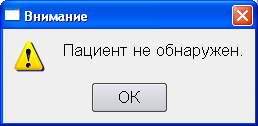
\includegraphics[width = 0.3\textwidth ,keepaspectratio]{cl_nofind}
 \caption{Сообщение о безрезультатном поиске}
 \label{img_cl_nofind}
\end{figure} 

\subsubsection{Поиск по штрих-коду}

В \tmis~предусмотрена возможность поиска по штрих-коду страхового полиса пациента 

\begin{prim}
 Данная функция реализована для определенных регионов РФ.
\end{prim}

\begin{vnim}
Для использования возможности поиска по штрих-коду рабочее место должно быть оборудовано сканером штрих-кодов.
\end{vnim}

Для поиска по штрих-коду требуется нажать кнопку \btn{Считать штрих-код} , расположенную в секции 6. Откроется окно (Рисунок \ref{img_cl_barcodef}), в поле которого нужно считать штрих-код, используя сканер. По полученным данным штрих-кода будет осуществлен поиск регистрационной карточки пациента. Если карточка в картотеке пациентов отсутствует, то при регистрации новой карточки данные, полученные из штрих-кода, будут подставлены в соответствующие поля карточки.

\begin{figure}[ht]\centering
 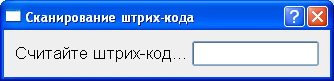
\includegraphics[width = 0.5\textwidth ,keepaspectratio]{cl_barcodef}
 \caption{Окно сканирования штрих-кода}
 \label{img_cl_barcodef}
\end{figure} 

\subsubsection {Поиск по данным универсальной электронной карты (УЭК)}

Аналогично предыдущему случаю, \tmis~позволяет поиск данных и регистрацию пациентов на основе УЭК пациента.

\begin{vnim}
 Для использования возможности поиска по данным УЭК рабочее место должно быть оборудовано карт-ридером.
\end{vnim}

Необходимо вставить УЭК в карт-ридер и нажать кнопку \btn{Считать с УЭК}, расположенную в секции 6. После непродолжительного ожидания будет осуществлен поиск регистрационной карточки пациента по данным УЭК. Если поиск не дал результатов, то при регистрации новой карточки, данные считанные с УЭК будут подставлены в соответствующие поля автоматически.

\subsubsection {Расширенный фильтр}

Вкладка \dm{Расширенный фильтр} содержит критерии фильтрации, предназначенные для формирования различных списков пациентов, поиска и выявления ошибок в заполнении регистрационных карточек.

На вкладке имеются следующие критерии поиска:
\begin{itemize}
 \item \dm{Автор} – поиск регистрационных карточек пациентов, зарегистрированных выбранным пользователем. Имя пользователя выбирается из списка.
 \item	\dm{Дата создания} – поиск регистрационных карточек пациентов, созданных в указанный период дат. Требуется указать две даты: дату начала и дату окончания периода для поиска.
 \item	\dm{Автор последнего изменения} – поиск регистрационных карточек пациентов, последние изменения в которые были внесены указанным пользователем. Имя пользователя выбирается из списка.
 \item	\dm{Дата последнего изменения} – поиск регистрационных карточек пациентов, измененных в указанный период дат. Требуется указать две даты: дату начала и дату окончания периода для поиска.
 \item	\dm{Возраст} – поиск пациентов, возраст которых удовлетворяет заданному интервалу. Необходимо указать границы начала и конца интервала, а так же для каждой границы выбрать единицу измерения (лет, месяцев, недель, дней). По умолчанию исчисление ведется в годах.
 \item \dm{По участку} – поиск пациентов, прикрепленных к указанному участку. Требуется выбрать тип прикрепления из списка и подразделение ЛПУ (участок) прикрепления в структуре ЛПУ.
 \item	\dm{По койкам} – поиск пациентов, зарегистрированных на койках в указанном отделении. Необходимо выбрать состояние регистрации из списка, а затем выбрать отделение из структуры ЛПУ. По умолчанию список формируется по всему ЛПУ.
 \item	Установка флажка \dm{Адрес} пуст позволяет найти регистрационные карточки пациентов, в которых не заполнен или не полностью заполнен адрес регистрации. В выборку так же попадают карточки, в которых адрес введен вручную БЕЗ использования справочника КЛАДР.
 \item \dm{Прикрепление} – поиск регистрационных карточек с заданным типом и видом прикрепления. Необходимо сначала выбрать тип прикрепления в верхнем поле («Постоянное», «Временное» или «Выбыл»). В зависимости от выбранного типа будет сформирован список видов прикрепления во втором поле. Если второе поле оставить незаполненным, сформируется список карточек с любым видом прикрепления указанного типа.
 \item	\dm{Прикрепление к ЛПУ} – поиск пациентов, прикрепленных к выбранному ЛПУ. ЛПУ выбирается из списка.
 \item \dm{Любое ЛПУ кроме базового} – поиск пациентов, прикрепленных к другим ЛПУ.
 \item	\dm{Период ВУТ} – поиск пациентов, имеющих листки временной нетрудоспособности в указанный период. Требуется указать две даты: дату начала и дату окончания периода для выборки.
\end{itemize}

Как и в случае использования вкладки \dm{Поиск}, для использования критерия поиска следует установить флажок \putx~слева от его названия. Для получения результатов поиска, необходимо нажать кнопку \btn{Применить}. Для того чтобы вернуться к полному списку пациентов, нужно нажать кнопку \btn{Сбросить} .

Возможно одновременное использование критериев поиска со вкладок \dm{Поиск} и \dm{Расширенный фильтр}.

\subsection{Регистрационная карточка пациента} \label{cl_card}

Регистрационная карточка пациента содержит всю персональную информацию о пациенте: его фамилию, имя, отчество, дату рождения, адрес, сведения о документах пациента, его страховых полисах, льготах, занятости и т.д. Вся эта информация должна вводиться регистратором с первичных документов пациента при первом обращении в ЛПУ. В момент регистрации пациента ему присваивается уникальный код, по которому его регистрационную карточку можно быстро найти в картотеке пациентов.

Регистрационная карточка пациента имеет вид, приведенный на рисунке \ref{img_cl_card}. В связи с большим объемом данных о пациенте, которые необходимо хранить, вся информация разбита на несколько вкладок. В верхней части окна отображается основные идентификационные данные пациента (ФИО, дата рождения, место рождения, пол, СНИЛС), которые видны на любой вкладке. При регистрации нового пациента, рекомендуется заполнять их в первую очередь.

\begin{figure}[ht]\centering
 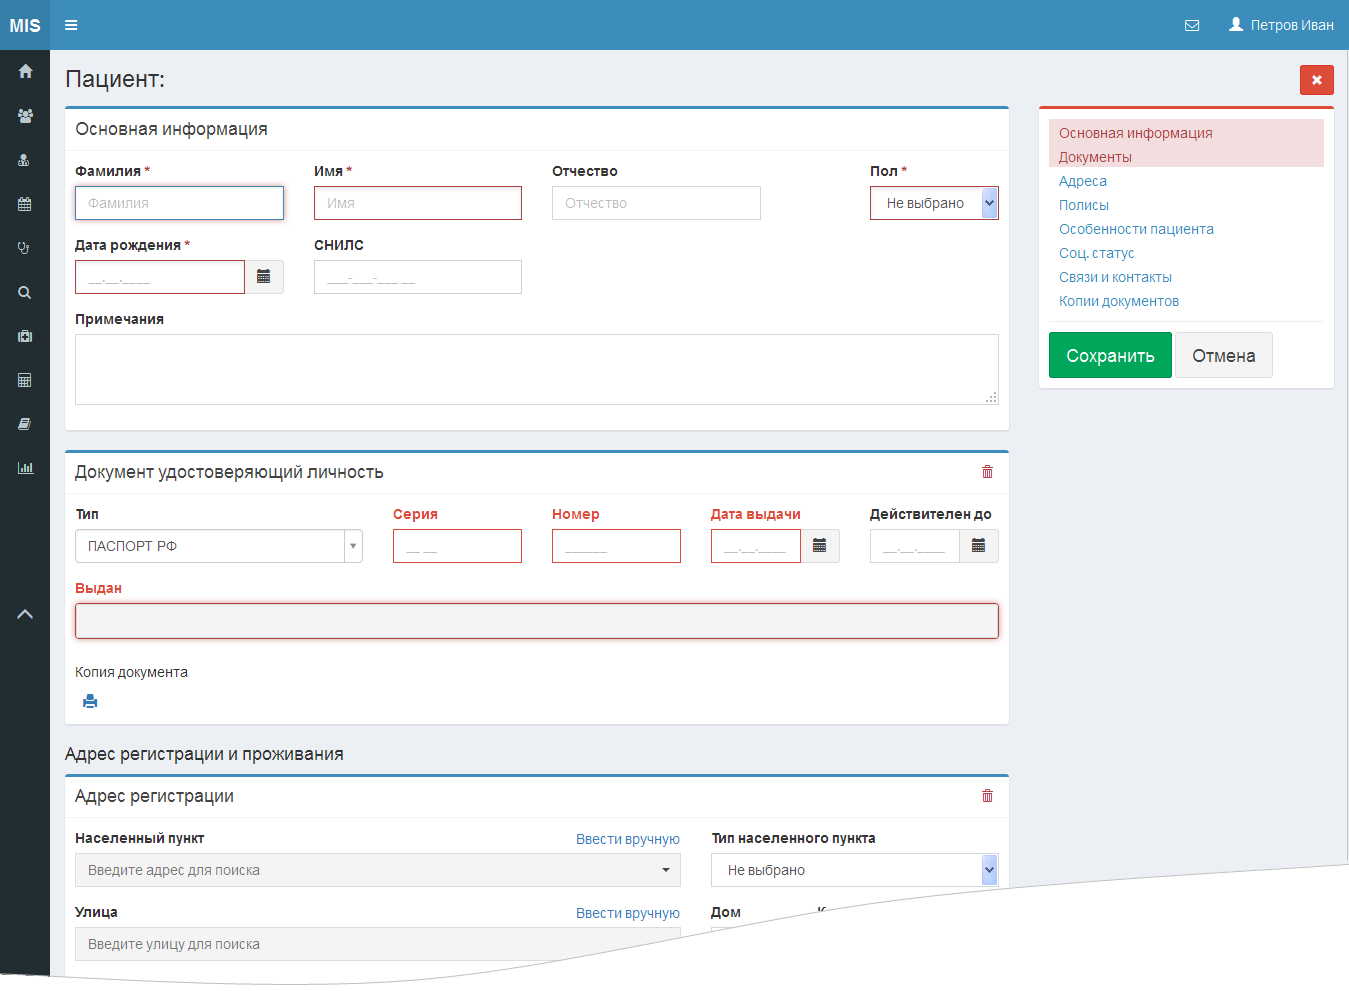
\includegraphics[width = 1\textwidth ,keepaspectratio]{cl_card}
 \caption{Регистрационная карточка пациента}
 \label{img_cl_card}
\end{figure} 

Поля \dm{Фамилия}, \dm{Имя}, \dm{Дата рождения}, \dm{Тип населенного пункта} (адреса регистрации и проживания) в окне регистрации пациента являются обязательными для заполнения. Они помечены символом <<*>> красного цвета.

Поле \dm{Дата рождения} может заполняться с клавиатуры или выбираться из календаря. При заполнении с клавиатуры дата вводится в формате <<ДД.ММ.ГГГГ>>, разделительные точки при вводе можно опустить. Т.е. ввод значения <<12041945>> равнозначен вводу <<12.04.1945>>. Для выбора даты из календаря, нужно нажать кнопку 
\includegraphics{sdown}  в конце поля. Аналогичным образом заполняются все даты в регистрационной карточке.

Значение поля \dm{Пол} может вводиться с клавиатуры или выбираться из списка с помощью мыши. В поле \dm{СНИЛС}, как и при вводе дат, достаточно ввести только цифры, разделительные тире будут вставлены автоматически. В случае использования системы за пределами РФ, на месте СНИЛС указывается индивидуальный номер гражданина, принятый в данной стране.

\subsubsection{Вкладка <<Паспортные данные>>}

Вкладка \dm{Паспортные данные} содержит основную регистрационную информацию пациента (сведения об адресе проживания, документе удостоверяющем личность и полисах медицинского страхования).

В регистрационной карточке существует возможность указания двух адресов для каждого пациента: адреса регистрации и адреса фактического проживания. Заполнение адреса рекомендуется выполнять с помощью всероссийского классификатора адресов КЛАДР (флажок \dm{КЛАДР} установлен по умолчанию). Только в случае, если найти адрес в справочнике не удалось, допускается снять флжок \dm{КЛАДР} и ввести адрес вручную в ставшую активной строку ввода. Поле \dm{Тип населенного пункта} необходимо для статистического учета и является обязательным для заполнения. В случае если адрес заполняется из справочника КЛАДР, в первом поле выбирается название населенного пункта, а во втором – название улицы. Список улиц изменяется в зависимости от выбранного населенного пункта. Выбор населенного пункта организован с помощью дерева. Сначала нужно выбрать регион и нажать кнопку <<+>> слева от его названия, затем в раскрывшемся списке выбрать район и раскрыть его аналогичным способом, затем выбрать населенный пункт двойным нажатием левой кнопки мыши.

\begin{prim}
Кнопка 
\includegraphics{srigth} слева от заголовка \dm{Адрес регистрации} позволяет скопировать адрес из предыдущей регистрационной карточки. Кнопка 
\includegraphics{sdown} справа от поля \dm{Тип населенного пункта} адреса проживания позволяет скопировать адрес проживания из адреса регистрации.
\end{prim}

В разделе \dm{Документ} указываются данные документа, удостоверяющего личность пациента. Как правило, для детей таким документом является свидетельство о рождении, а для взрослых – паспорт, однако, возможны и другие варианты. \dm{Тип документа} выбирается из справочника. Далее следует указать серию, номер документа, дату выдачи и срок действия, кем был выдан документ.

В случае если какие-то данные в документе не указаны (например, не все документы имеют номер серии или срок действия), соответствующие поля заполнять не нужно.

\begin{vnim}
Для заполнения серии документа выделено 2 отдельных поля, т.к. зачастую серия состоит из двух групп символов. Будьте внимательны при вводе номера документа, часто его ошибочно вводят во второе поле для указания серии документа!
\end{vnim}
  
В разделе \dm{Полис ОМС} указываются данные действующего полиса обязательного медицинского страхования. Необходимо указать серию и номер страхового полиса, дату выдачи и срок действия. В строке \dm{СМО} требуется выбрать из списка название СМО и в следующем поле – тип полиса. Если название СМО отсутствует в списке, то это поле нужно оставить пустым, а ниже, в поле \dm{Название}, ввести его вручную. В поле \dm{Примечание} можно внести любые дополнительные сведения о полисе ОМС (например, <<данные внесены на основании ксерокопии>>).

Если региональный ФОМС предоставляет ЛПУ online-сервис для проверки полисов ОМС пациентов, то в разделе \dm{Полис ОМС} становится доступной кнопка \btn{Искать}. Для проверки следует заполнить данные полиса ОМС и нажать кнопку \btn{Искать}. Будет выполнен запрос на проверку данных к сервису ТФОМС и после получения ответа, он появится на экране в виде сообщения. При наличии возможности проверки полиса, рекомендуется максимально использовать ее, так как это позволяет избежать большого числа ошибок при заполнении данных пациента и, как следствие, снизить число отказов в оплате со стороны СМО.

Раздел \dm{Полис ДМС} заполняется аналогично разделу \dm{Полис ОМС}, но хранит данные о действующем полисе ДМС пациента.

\begin{prim}
При изменении данных полиса или документа, удостоверяющего личность, на вкладке \dm{Паспортные данные}, ранее введенные данные не теряются. Все ранее зарегистрированные для пациента полисы  и документы, удостоверяющие личность, можно найти на вкладке \dm{Документы} (см.раздел \ref{cl_docs})
\end{prim}

\subsubsection{Вкладка <<Соц.статус>>} \label{cl_socst}

На данной вкладке расположен ряд дополнительных сведений о пациенте, которые используются, в первую очередь для статистического учета (Рисунок \ref{img_cl_socst}). Заполнение информации о социальных статусах является обязательным. Состав классов соц.статусов может отличаться в различных ЛПУ.

Порядок заполнения таблицы соц.статусов должен быть следующий:
\begin{enumerate}
 \item Двойным щелчком левой кнопки мыши на пустой ячейке в столбце \dm{Класс} нужно активизировать список классов.
 \item Из полученного списка так же двойным щелчком требуется выбрать название класса.
 \item В ячейке \dm{Тип} необходимо выбрать значение класса соц.статусов.
 \item Если известна дата приобретения статуса, нужно указать ее в ячейке \dm{Дата начала}.
 \item Если известен срок действия статуса, нужно указать его в ячейке \dm{Дата завершения}.
 \item Желательно ввести данные о документе, подтверждающем соц.статус в нижней части окна (Рисунок \ref{img_cl_socst}).
 \item Требуется повторить шаги 1 – 6 для ввода значений других классов соц.статусов.
\end{enumerate}

\begin{figure}[ht]\centering
 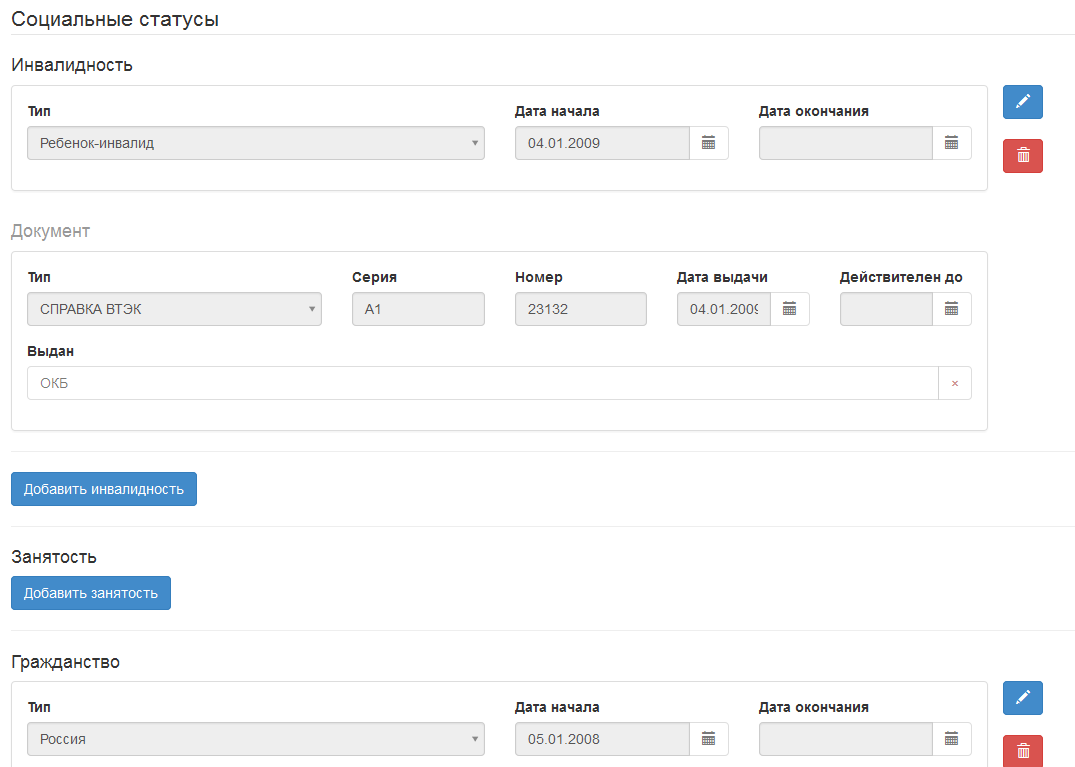
\includegraphics[width = 1\textwidth ,keepaspectratio]{cl_socst}
 \caption{Регистрационная карточка пациента. Вкладка <<Соц.статус>>}
 \label{img_cl_socst}
\end{figure} 

Необходимость ввода данных о документе, подтверждающем соц.статус, определяется соображениями целесообразности и рабочими инструкциями в каждом ЛПУ. Например, для класса <<Инвалидность>> ввод информации о подтверждающем документе является обязательным, а для класса <<Занятость>> – не имеет смысла.

\begin{prim}
Данные обо всех документах, подтверждающих соц.статусы можно так же просмотреть на вкладке \dm{Документы}.
\end{prim}
 
Для удаления записи из таблицы соц.статусов нужно щелкнуть правой кнопкой мыши на этой записи и в контекстном меню выбрать пункт \dm{Удалить текущую строку}.

\begin{prim}
Для удаления нескольких записей одновременно необходимо выделить эти записи с помощью мыши, удерживая клавиши \keys{Shift} или \keys{Ctrl} на клавиатуре, либо с помощью стрелок на клавиатуре и клавиши \keys{Shift}, затем щелкнуть правой кнопкой мыши внутри области выделения и выбрать пункт меню \dm{Удалить выделенные строки}.
\end{prim}

\subsubsection{Вкладка <<Прикрепление>>}

Вкладка \dm{Прикрепление} содержит сведения о ЛПУ прикрепления пациента (Рисунок \ref{img_cl_prikr}).

\begin{figure}[ht]\centering
 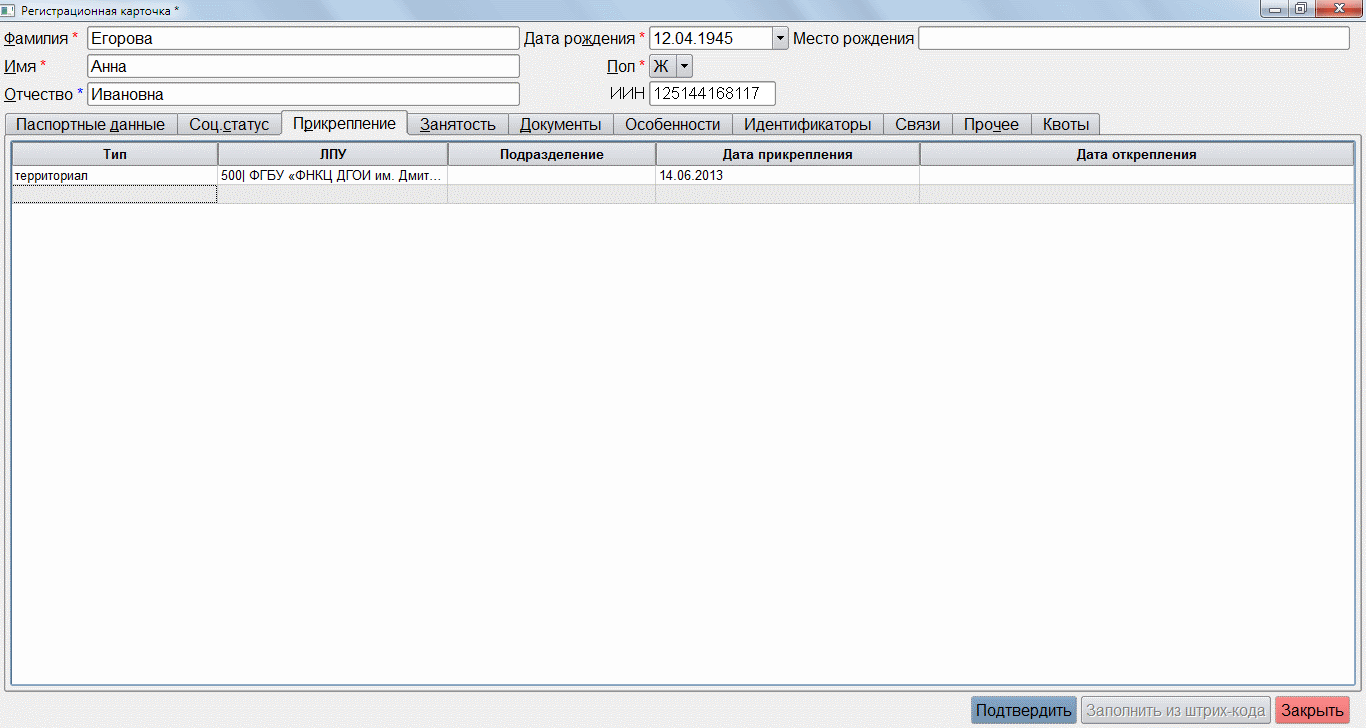
\includegraphics[width = 1\textwidth ,keepaspectratio]{cl_prikr}
 \caption{Регистрационная карточка пациента. Вкладка <<Прикрепление>>}
 \label{img_cl_prikr}
\end{figure} 

Порядок добавления данных о прикреплении следующий:
\begin{enumerate}
 \item Если в таблице уже присутствуют записи о прикреплении, то требуется заполнить \dm{Дату окончания} предыдущей записи о прикреплении.
 \item Двойным щелчком левой клавиши мыши на пустой ячейке в столбце \dm{Тип} нужно активизировать список прикрепления. Из появившегося списка необходимо выбрать тип прикрепления.
 \item В ячейке \dm{ЛПУ} необходимо выбрать название ЛПУ прикрепления из списка.
 \item В ячейке \dm{Подразделение} можно указать название подразделения, если прикрепление осуществляется к конкретному подразделению. Если прикрепление действительно в рамках всего ЛПУ, то ячейку заполнять не нужно.
 \item В ячейке \dm{Дата начала} автоматически ставится текущая дата, но ее можно изменить в соответствии с данными о прикреплении.
 \item Ячейку \dm{Дата окончания} заполнять не обязательно. В случае, если она остается пустой, считается, что прикрепление бессрочно.
\end{enumerate}
 
Удаление записей производится аналогично удалению записей соц.статусов с помощью контекстного меню (см. раздел \ref{cl_socst})

\subsubsection{Вкладка <<Занятость>>}

Вкладка \dm{Занятость} содержит информацию о месте работы или учебы пациента, профессиональных вредностях и неблагоприятных факторах, связанных с работой пациента (Рисунок \ref{img_cl_workpl}). Для неорганизованных пациентов этот раздел остается пустым. Чтобы поля на вкладке \dm{Занятость} были доступны для ввода и редактирования, необходимо добавить хотя бы одну запись на вкладке \dm{Соц.статус}.

\begin{figure}[ht]\centering
 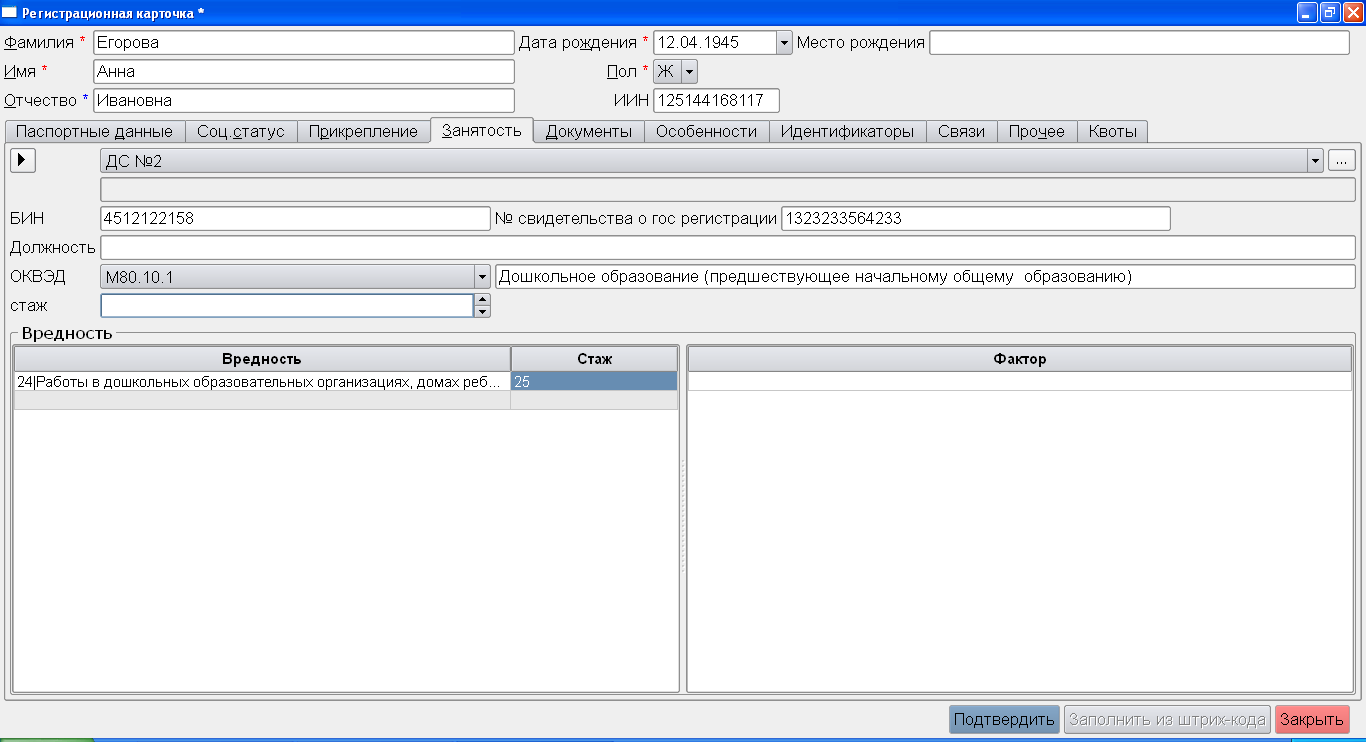
\includegraphics[width = 1\textwidth ,keepaspectratio]{cl_workpl}
 \caption{Регистрационная карточка пациента. Вкладка <<Занятость>>}
 \label{img_cl_workpl}
\end{figure} 

Название организации – места работы пациента можно выбрать из справочника или ввести вручную. Выбор названия из справочника осуществляется в поле 1 (Рисунок \ref{img_cl_workpl}). После заполнения поля 1, поле 2 становится недоступным для ввода, поля \dm{ИНН} и \dm{ОГРН} заполняются автоматически из справочника, в поле \dm{ОКВЭД} список выбора ограничивается кодом ОКВЭД, заданным для данной организации в справочнике. Если поле 1 не заполнено (название организации не найдено в справочнике), то допускается свободный ввод названия организации в поле 2. При этом поля \dm{ИНН} и \dm{ОГРН} остаются пустыми, в поле \dm{ОКВЭД} содержится полный список кодов.

\begin{prim}
Если значительная часть пациентов, обслуживаемых ЛПУ, работает в одной и той же организации рекомендуется внести ее в справочник. Так же рекомендуется вводить в справочник наиболее часто встречающиеся места работы пациентов. Это позволит повысить скорость регистрации пациентов.
\end{prim}
 
После того как выбрано или введено название организации, требуется указать должность пациента, при наличии информации выбрать код ОКВЭД и ввести стаж работы на данной позиции в годах. 

При наличии на работе пациента вредностей и факторов риска, необходимо заполнить раздел \dm{Вредность} в нижней части. Для этого двойным щелчком левой кнопки мыши на пустой ячейке в столбце \dm{Вредность} нужно активизировать список вредностей, выбрать значение из списка и в следующей ячейке ввести срок работы с указанной вредностью в годах. Таким образом, можно указать несколько профессиональных вредностей для одного пациента. Аналогичным способом заполняются факторы риска, но указание стажа работы здесь не требуется.

Удаление записей о профессиональных вредностях и факторах риска осуществляется с помощью контекстного меню (см. подробное описание в разделе \ref{cl_socst})

С помощью кнопки 3 (Рисунок \ref{img_cl_workpl}) предусмотрен поиск организации в справочнике по заданным параметрам. При этом открывается окно (Рисунок \ref{img_cl_org_find}), где требуется указать один или несколько параметров поиска. В случае если задается сразу несколько параметров поиска, связаны они будут по <<И>>, т.е. будет осуществлен поиск организаций, для которых выполняются все заданные условия одновременно.

\begin{figure}[ht]\centering
 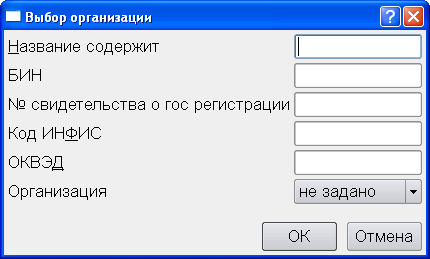
\includegraphics[width = 0.4\textwidth ,keepaspectratio]{org_find}
 \caption{Окно параметров поиска организации}
 \label{img_cl_org_find}
\end{figure} 

В поле \dm{Название содержит} можно указать часть названия организации, регистр при этом не учитывается; в поле \dm{Организация} из списка можно выбрать тип организации (СМО, ЛПУ или организация). После того, как параметры поиска заданы, нужно нажать кнопку \btn{OK} . Если в результате поиска найдена единственная организация, она автоматически будет подставлена в поле 1 (Рисунок \ref{img_cl_workpl}). Если поиск не дал результатов или найдено более одной организации, удовлетворяющей условиям, появится список найденных организаций. Двойной щелчок левой кнопкой мыши на выбранной записи позволяет подставить данное значение в поле 1 (Рисунок \ref{img_cl_workpl}).

\begin{prim}
 Кнопка 4 (Рисунок \ref{img_cl_workpl}) позволяет скопировать данные о месте работы пациента из предыдущей регистрационной карточки.
\end{prim}

\subsubsection{Вкладка <<Документы>>} \label{cl_docs}

Как уже упоминалось ранее, данная вкладка содержит информацию обо всех документах, которые когда-либо регистрировались для данного пациента, т.е. историю изменений документов пациента (Рисунок \ref{img_cl_docs}). Все документы пациента, в зависимости от их типа, распределены по 3 вкладкам:
\begin{itemize}
 \item \dm{Идентификация} – документы, удостоверяющие личность пациента;
 \item	\dm{Полисы} – полисы ОМС и ДМС;
 \item	\dm{Соц.статус} – документы, зарегистрированные во вкладке \dm{Соц.статус}.
\end{itemize}

\begin{figure}[ht]\centering
 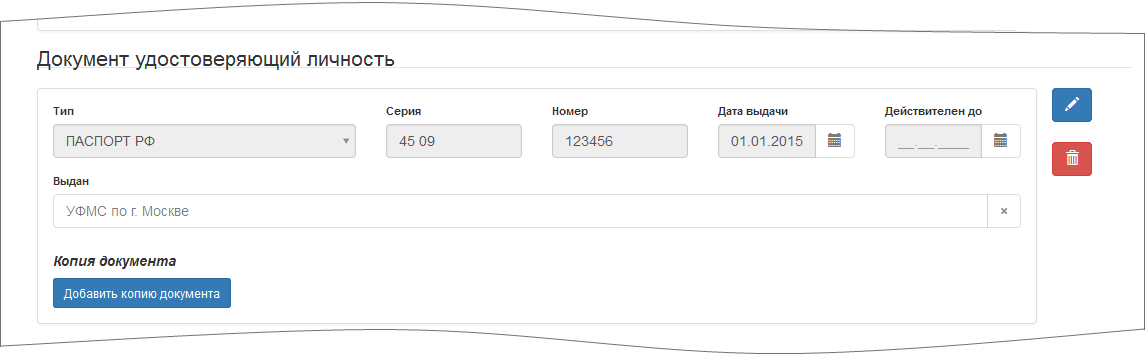
\includegraphics[width = 1\textwidth ,keepaspectratio]{cl_docs}
 \caption{Регистрационная карточка пациента. Вкладка <<Документы>>}
 \label{img_cl_docs}
\end{figure} 

Редактирование данных на данной вкладке невозможно. Информация предназначена только для просмотра. Для получения подробных сведений о записи следует щелкнуть правой кнопкой мыши по выбранной записи и в контекстном меню выбрать пункт \dm{Свойства записи}. Откроется окно, где будут указаны сведения о дате создания и последнего редактирования записи, а так же имя пользователя (ей), выполнившего(их) данные операции.

\subsubsection{Вкладка <<Особенности>>}

Вкладка \dm{Особенности} содержит жизненно-важные параметры, необходимые для оказания медицинской помощи (витальную информацию): группу крови, аллергии и медикаментозную непереносимость (Рисунок \ref{img_cl_vit}). 

\begin{figure}[ht]\centering
 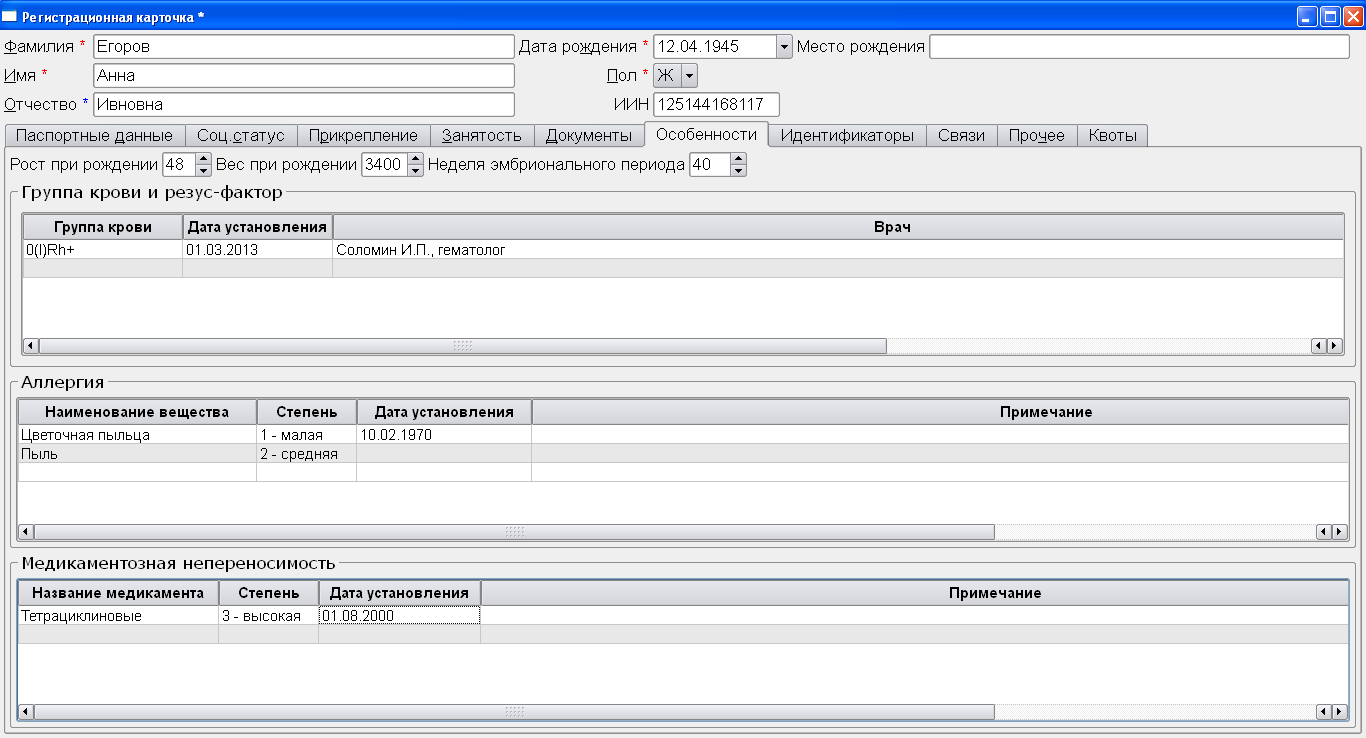
\includegraphics[width = 1\textwidth ,keepaspectratio]{cl_vit}
 \caption{Регистрационная карточка пациента. Вкладка <<Особенности>>}
 \label{img_cl_vit}
\end{figure} 

 Поля \dm{Рост при рождении} и \dm{Вес при рождении}, \dm{Неделя эмбрионального периода} заполняются для детей. Рост указывается в сантиметрах, вес -- в граммах. 
 
 В подразделе \dm{Группа крови и резус-фактор} хранится история ведения информации о группе крови пациента. Если группа крови известна на этапе регистрации пациента, то ее необходимо внести в данный раздел, активировав ячейку \dm{Группа крови} двойным щелчком мыши. В поле \dm{Дата установления} нужно указать дату установления группы крови, по умолчанию оно заполняется текущей датой, в поле \dm{Примечание} можно указать другую важную информацию, для которой не предусмотрено отдельных полей. Удаление записей из данного подраздела невозможно. В случае ошибочно введенного значения необходимо добавить в таблицу новую запись, содержащую правильное значение.

Подразделы \dm{Аллергия} и \dm{Медикаментозная непереносимость} заполняются по одному и тому же принципу. Необходимо щелкнуть левой кнопкой мышки по пустой ячейке в колонке \dm{Наименование вещества (Наименование медикамента)} и ввести описание аллергена, например <<пыль>> или <<доксициклин>>, в ячейке \dm{Степень} выбрать степень аллергической реакции, в ячейке \dm{Дата установления} ввести дату установления аллергии (медикаментозной непереносимости). По умолчанию, в качестве даты установления указывается текущая дата. В поле \dm{Примечание}, можно указать дополнительные сведения относительно реакции. В каждом подразделе может содержаться любое количество записей.

Удаление записей из подразделов \dm{Аллергия} и \dm{Медикаментозная непереносимость} выполняется с помощью контекстного меню (подробное описание см. в разделе \ref{cl_socst})

\subsubsection{Вкладка <<Идентификаторы>>}

\begin{figure}[ht!]\centering
 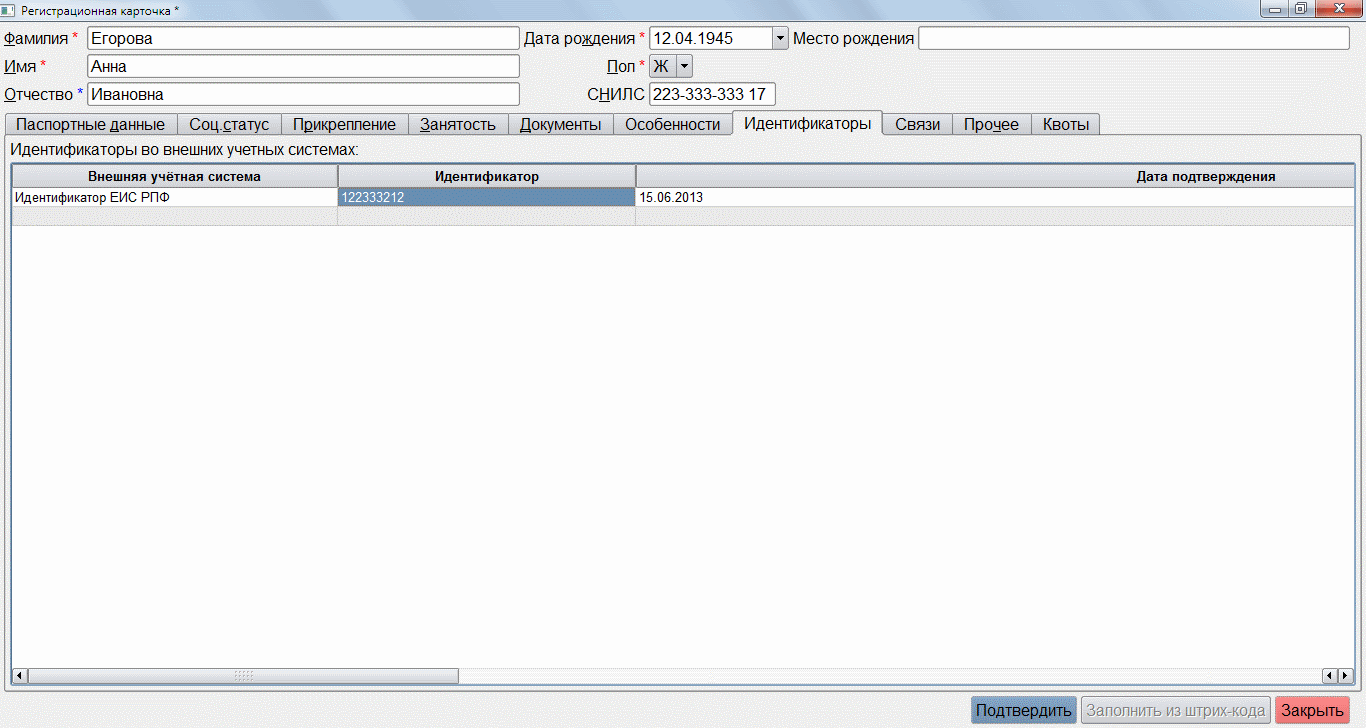
\includegraphics[width = 1\textwidth ,keepaspectratio]{cl_dopid}
 \caption{Регистрационная карточка пациента. Вкладка <<Идентификаторы>>}
 \label{img_cl_dopid}
\end{figure} 

Данная вкладка содержит информацию обо всех идентификаторах пациента в других внешних системах (Рисунок \ref{img_cl_dopid}). Для добавления идентификатора требуется двойным щелчком левой кнопки мыши по пустой ячейке в колонке \dm{Внешняя учетная система} активизировать список идентификаторов, выбрать из списка нужный вид идентификатора, ввести значение идентификатора в ячейку \dm{Идентификатор}, заполнить \dm{Дату подтверждения}. Можно ввести любое количество идентификаторов, но лишь один каждого вида. 

\subsubsection{Вкладка <<Связи>>}

Вкладка \dm{Связи} содержит указатели на регистрационные карточки родственников пациента (Рисунок \ref{img_cl_connect}). В верхней части окна указываются связи от родителей (или опекунов) к детям, в нижней части – от детей к родителям (опекунам). Т.е. если пациент является родителем, то связи с его детьми должны устанавливаться в верхней половине окна. При создании связи, в карточку второго пациента она добавляется автоматически в противоположный раздел.

\begin{prim}
 Для некоторых ЛПУ регистрация родителя или опекуна в карточке пациента является обязательной, если у пациента отсутствует собственный полис ОМС (Определяется настройками системы).
\end{prim}

\begin{figure}[ht!]\centering
 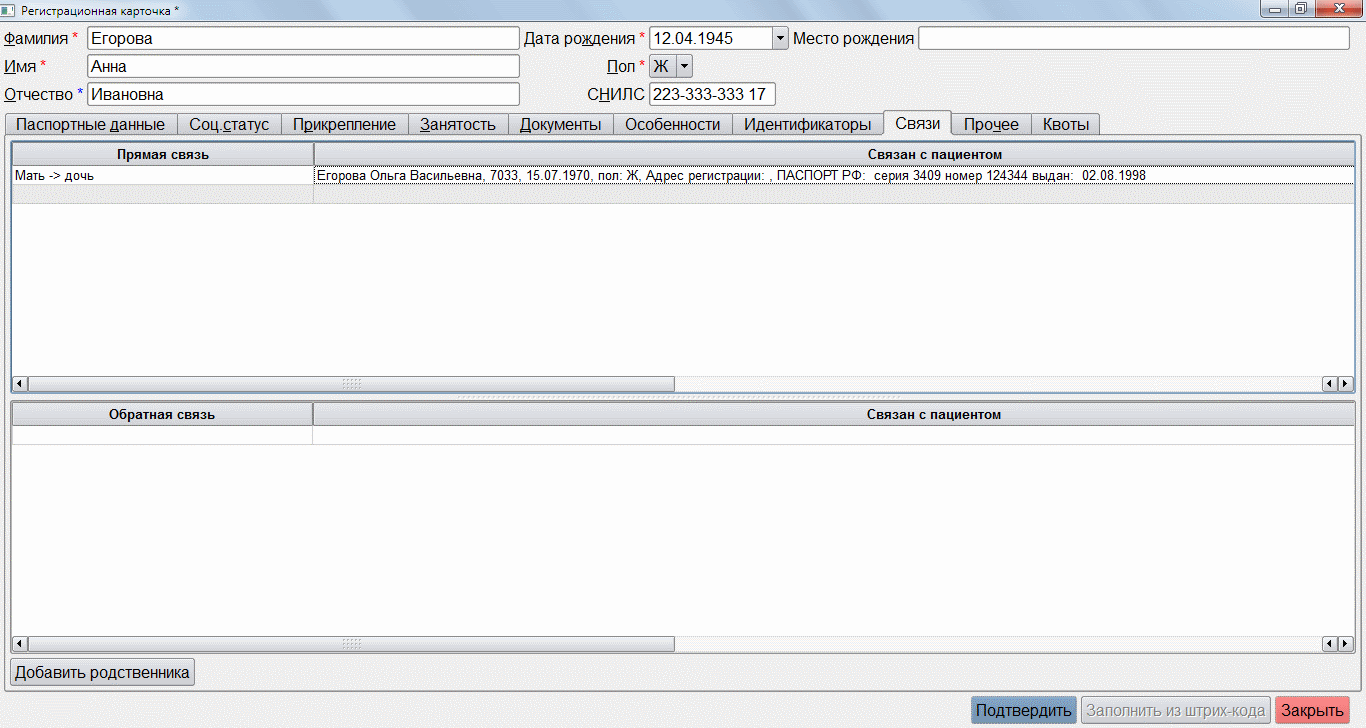
\includegraphics[width = 1\textwidth ,keepaspectratio]{cl_connect}
 \caption{Регистрационная карточка пациента. Вкладка <<Связи>>}
 \label{img_cl_connect}
\end{figure} 

Для добавления связи необходимо двойным щелчком левой кнопки мыши в свободной ячейке колонки \dm{Прямая связь (Обратная связь)} активировать список видов связей, затем выбрать из списка вид связи. Если пациент, с которым организуется связь, уже зарегистрирован в \tmis, нужно вызвать окно поиска, которое раскрывается по кнопке 
\includegraphics{sdown}, расположенной в конце ячейки \dm{Связан с пациентом}, ввести в поля параметры поиска (например, ФИО пациента) и нажать кнопку \btn{Применить} (Рисунок \ref{img_cl_connectf}). На экране появится список пациентов, соответствующих параметрам поиска. Двойным щелчком левой кнопки мыши требуется выбрать из него искомого пациента. Данные пациента будут автоматически вставлены в ячейку \dm{Связан с пациентом}.

\begin{figure}[ht!]\centering
 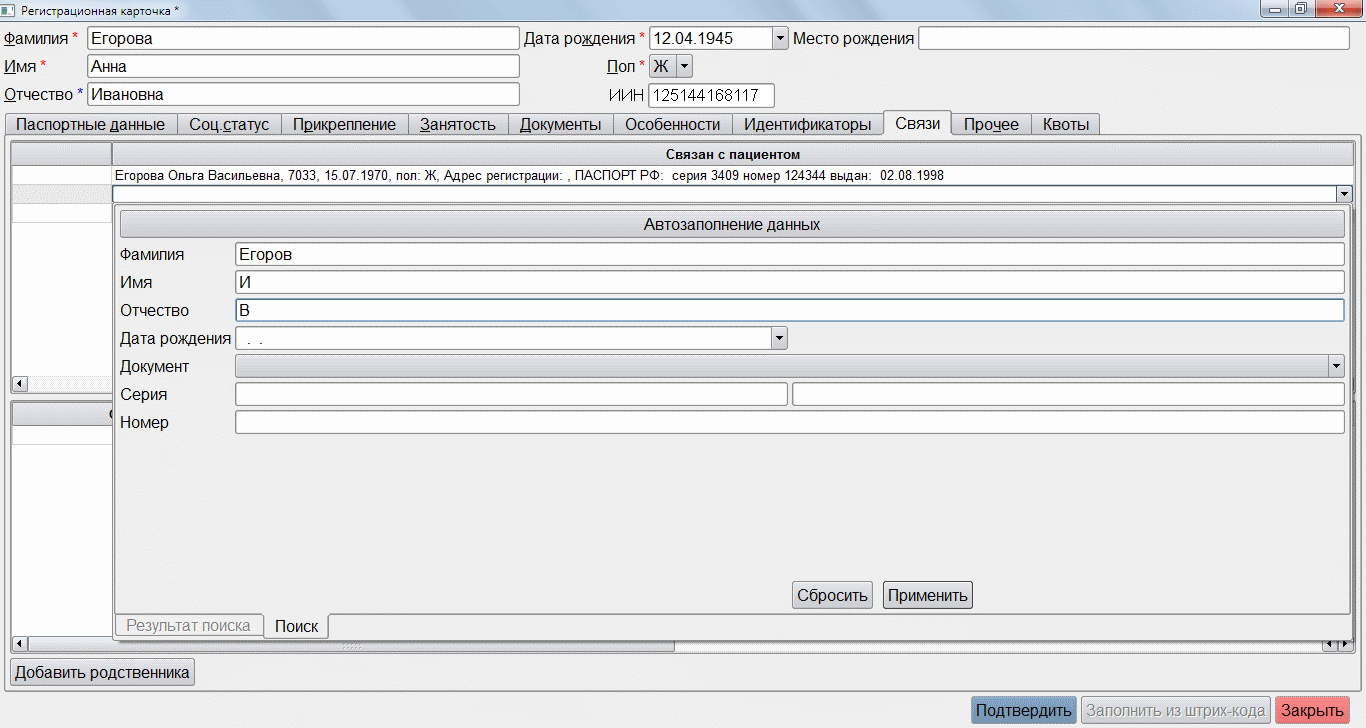
\includegraphics[width = 1\textwidth ,keepaspectratio]{cl_connectf}
 \caption{Окно поиска пациента для организации связи}
 \label{img_cl_connectf}
\end{figure} 

Если пациент, с которым организуется связь, не был ранее зарегистрирован в \tmis, можно зарегистрировать его, нажав кнопку \btn{Добавить родственника} в левом нижнем углу окна. Откроется новая регистрационная карточка пациента, которую необходимо заполнить данными родственника. После сохранения этой карточки, в карту текущего пациента будет добавлена связь с новым пациентом.

Для удаления записи о связи необходимо щелкнуть по ней правой кнопкой мыши и в раскрывшемся меню выбрать пункт \dm{Удалить текущую запись}.

Для редактирования регистрационной карточки связанного пациента нужно щелкнуть правой кнопкой мыши по соответствующей записи и в появившемся контекстном меню выбрать пункт \dm{Редактировать}. Откроется регистрационная карточка связанного пациента, доступная для редактирования.

\subsubsection{Вкладка <<Прочее>>}

Здесь содержится дополнительная информация о пациентах, которая не была учтена в других вкладках (Рисунок \ref{img_cl_other}). На этой вкладке можно хранить контактные данные пациента: номера телефонов, факсов, данные контактных лиц и т.п., а так же любую другую информацию в поле \dm{Примечание}.

\begin{figure}[ht]\centering
 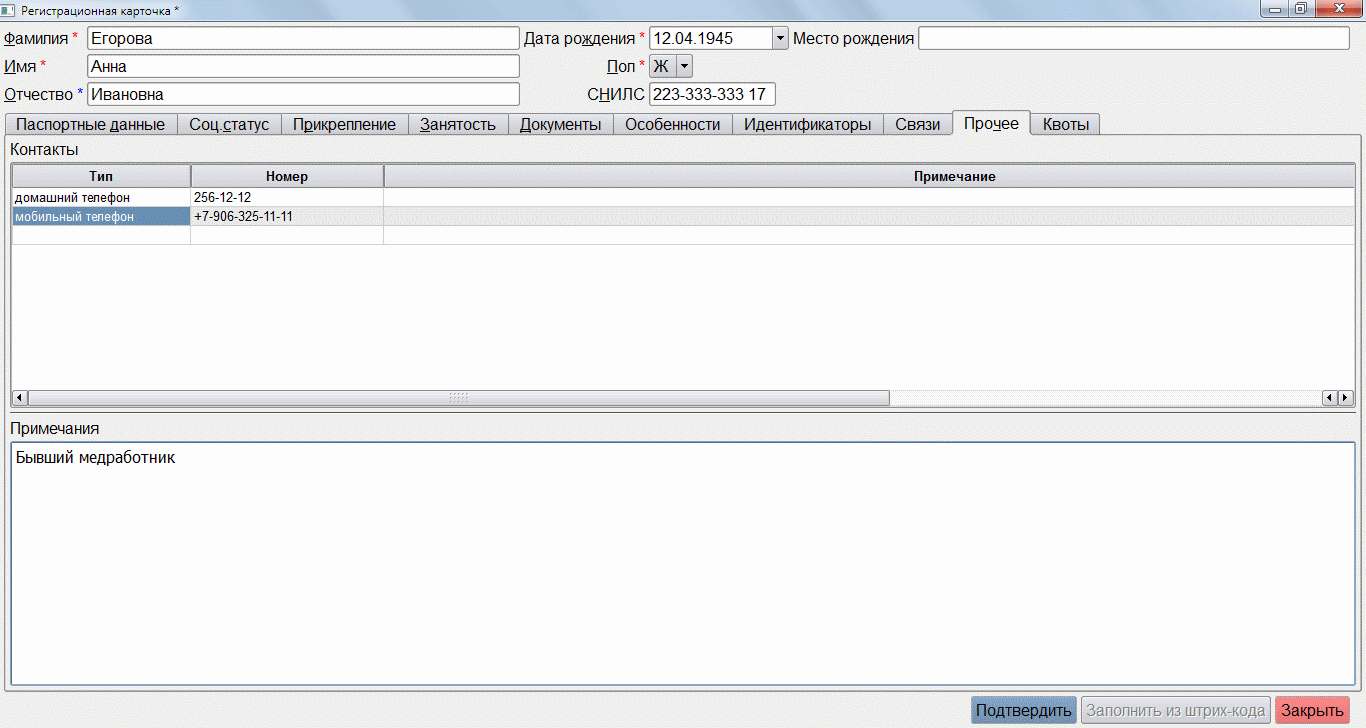
\includegraphics[width = 1\textwidth ,keepaspectratio]{cl_other}
 \caption{Регистрационная карточка пациента. Вкладка <<Прочее>>}
 \label{img_cl_other}
\end{figure} 

Для заполнения подраздела \dm{Контакты} требуется двойным щелчком левой кнопки мыши в пустой ячейке колонки \dm{Тип} активировать список типов контактов, затем выбрать из списка одно из значений, после чего в ячейке \dm{Номер} ввести номер соответствующего телефона, факса, адрес электронной почты и т.п. В ячейке \dm{Примечание} подраздела \dm{Контакты} можно указать любую дополнительную информацию относительно контакта, например, имена родственников и т.д.

Для удаления записи с контактной информацией необходимо щелкнуть по ней правой кнопкой мыши и в раскрывшемся меню выбрать пункт \dm{Удалить текущую запись}.

\subsubsection{Вкладка <<Квоты>>}

Вкладка содержит данные о выделенных пациенту квотах на высокотехнологичную медицинскую помощь. 

\subsection{Регистрация нового пациента} \label{cl_new}

Для регистрации нового пациента необходимо в главном меню выбрать пункт \dm{Работа \str Обслуживание пациентов}, после чего нажать кнопку \btn{Регистрация (F9)}  в нижней части открывшегося окна или нажать клавишу \keys{F9} на клавиатуре.

\begin{vnim}
Перед началом регистрации нового пациента необходимо убедиться, что данный пациент не был зарегистрирован ранее. Для этого рекомендуется воспользоваться поиском (см. раздел \ref{cl_find})
\end{vnim}

\begin{vnim}
Если кнопка регистрации не видна на экране, то необходимо выполнить переход в нижнюю часть окна, используя полосу прокрутки справа, или колесо прокрутки мыши. Для ускорения работы рекомендуется использовать клавишу \keys{F9} на клавиатуре.
\end{vnim}
 
После нажатия указанной кнопки или клавиши откроется окно \dm{Регистрационная карточка}, содержащее незаполненные поля. В них необходимо ввести все данные пациента в соответствии с разделом \ref{cl_card} <<Регистрационная карточка пациента>>. Для сохранения введенных данных нужно нажать кнопку \btn{Подтвердить}.

При попытке закрыть карточку без сохранения данных на экране появится окно (Рисунок \ref{img_cl_qq}). Если регистрационную карточку требуется сохранить, то нужно нажать кнопку \btn{Не выходить} , а затем кнопку \btn{Подтвердить}  в окне \dm{Регистрационная карточка}. Если сохранение карточки не требуется, нужно нажать кнопку \btn{Выйти без сохраниения}.

\begin{figure}[ht]\centering
 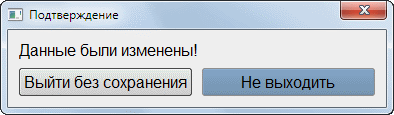
\includegraphics[width = 0.5\textwidth ,keepaspectratio]{cl_qq}
 \caption{Запрос подтверждения выхода без сохранения}
 \label{img_cl_qq}
\end{figure} 

\subsection{Редактирование регистрационной карточки пациента}

Данные, введенные в регистрационную карточку пациента, не являются статичными, их можно динамически изменять в соответствии с изменениями первичных документов у пациента. При изменении каких-либо документов у пациента, его социального статуса, выявлении новых особенностей и т.п., требуется открыть регистрационную карточку пациента на редактирование и внести в нее соответствующие изменения. 

Для редактирования регистрационной карточки пациента, нужно найти ее в картотеке пациентов и установить на ней курсор (щелкнуть левой кнопкой мыши). Для поиска рекомендуется использовать фильтрацию данных (см. раздел \ref{cl_find}) После того, как в верхней части окна появились данные искомого пациента, можно нажать кнопку \btn{Редактировать (F4)}  или клавишу \keys{F4} на клавиатуре.

\begin{vnim}
Если кнопка редактирования не видна на экране, то необходимо выполнить переход в нижнюю часть окна, используя полосу прокрутки справа, или колесо прокрутки мыши. Для ускорения работы рекомендуется использовать клавишу \keys{F4} на клавиатуре.
\end{vnim}
 
Откроется окно \dm{Регистрационная карточка}, содержащее ранее введенные данные о пациенте. Требуется внести изменения в соответствующие поля и сохранить их, нажав кнопку \btn{Подтвердить}. Заполнение полей регистрационной карточки подробно рассмотрено в разделе \ref{cl_card} <<Регистрационная карточка пациента>>.

Если были изменены данные документа, удостоверяющего личность, полиса пациента или документы, подтверждающие соц.статус, то данные старого документа можно найти на вкладке \dm{Документы} регистрационной карточки пациента. 
На вкладке \dm{Идентификаторы} регистрационной карточки невозможно изменение значения идентификатора. Если идентификатор внесен ошибочно, требуется удалить эту запись и добавить заново правильный идентификатор.

Для всех записей в табличном представлении (такие как соц.статусы, прикрепления, вредности и т.п.) можно посмотреть информацию о том, кто и когда ее создал, и кем и когда были сделаны последние изменения. Для этого требуется щелкнуть правой кнопкой мыши на интересующей записи и в появившемся контекстном меню выбрать пункт \dm{Свойства записи}. После этого откроется окно (Рисунок \ref{img_cl_propz}), содержащее сведения о создании и редактировании записи.

\begin{figure}[ht]\centering
 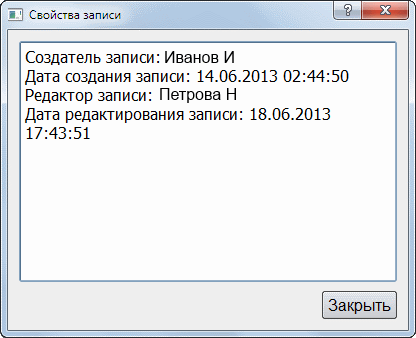
\includegraphics[width = 0.4\textwidth ,keepaspectratio]{cl_propz}
 \caption{Окно свойств записи}
 \label{img_cl_propz}
\end{figure} 

\subsection{Вывод на печать медицинских документов пациента}

Из картотеки пациентов можно распечатать ряд медицинских документов пациента. Для этого, находясь в окне картотеки пациентов, требуется выбрать пациента из списка и щелкнуть по нему левой кнопкой мыши. Для поиска нужного пациента рекомендуется воспользоваться фильтрами (см. раздел \ref{cl_find}) После того как пациент выбран, нужно нажать кнопку \btn{Печать (F6)} в нижней части окна (если кнопки не видны, рекомендуется воспользоваться полосами прокрутки). В появившемся меню (Рисунок \ref{img_cl_printm}) требуется выбрать пункт \dm{Напечатать талон}. Раскроется следующее меню, где нужно выбрать название медицинского документа, который следует напечатать, например \dm{Медицинская карта амбулаторного пациента}. Откроется окно предварительного просмотра обложки амбулаторной карты пациента (Рисунок \ref{img_cl_printing}). Для отправки документа на принтер, требуется нажать кнопку \btn{Печать} , для сохранения документа в файл – кнопку \btn{Сохранить} , при этом откроется диалоговое окно, где нужно указать имя, под которым будет сохранен файл, и выбрать папку для сохранения и тип файла.

\begin{figure}[ht]\centering
 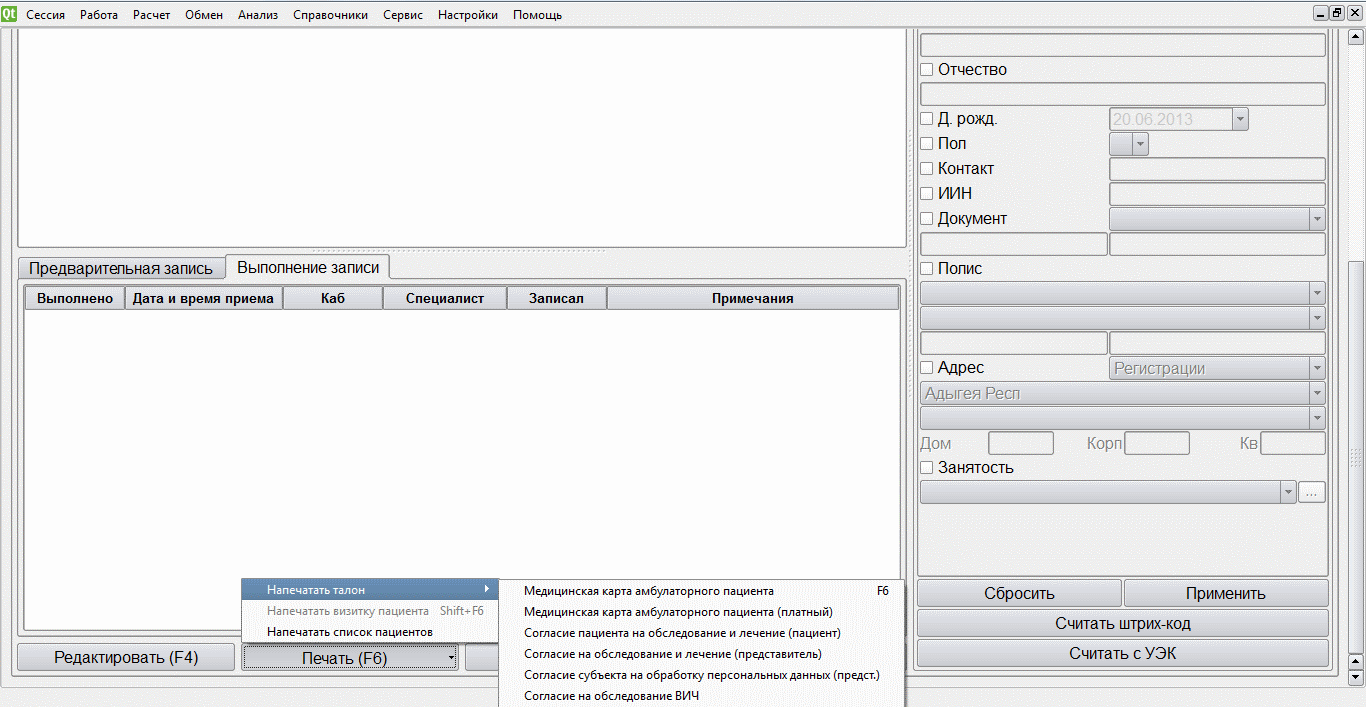
\includegraphics[width = 1\textwidth ,keepaspectratio]{cl_printm}
 \caption{Печать медицинских документов}
 \label{img_cl_printm}
\end{figure} 

\begin{figure}[ht]\centering
 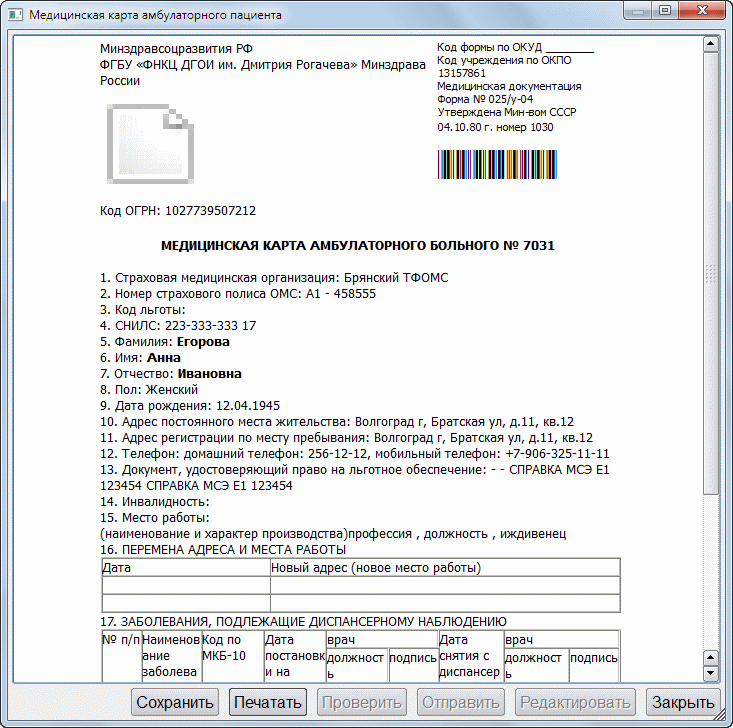
\includegraphics[width = 0.9\textwidth ,keepaspectratio]{cl_printp}
 \caption{Окно предварительного просмотра печатной формы}
 \label{img_cl_printing}
\end{figure} 

Тем же способом можно распечатать любой документ, присутствующий в меню, для выбранного пациента. Состав пунктов меню может отличаться в каждом ЛПУ.

Как правило, выделяется один наиболее часто используемый печатный документ, который вызывается по клавише \keys{F6}. Для него установлена соответствующая отметка в меню (на рисунке \ref{img_cl_printm} это <<Медицинская карта амбулаторного пациента>>). При нажатии клавиши \keys{F6} сразу открывается окно предварительного просмотра печатной формы данного документа, что позволяет сократить время, затрачиваемое на вызов печати документа.

\subsection{Печать списка пациентов}

Из картотеки пациентов можно так же распечатать список пациентов, отобранных по определенным критериям с помощью фильтра. Для этого нужно нажать кнопку \btn{Печать (F6)}  и выбрать пункт меню \dm{Напечатать список пациентов}. Откроется окно предварительного просмотра печати списка пациентов. Для печати списка требуется нажать кнопку \btn{Печать}, для сохранения списка в файл – кнопку \btn{Сохранить} , при этом откроется диалоговое окно, где нужно указать имя, под которым будет сохранен файл, и выбрать папку для сохранения.

